\begin{figure}[H]
\begin{center}
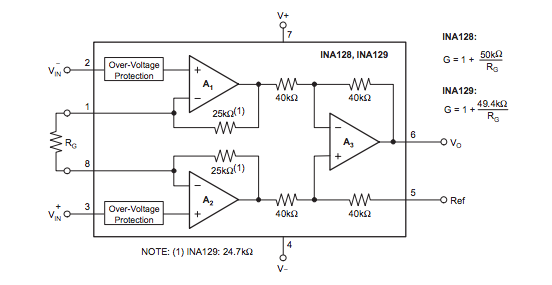
\includegraphics[width=8cm]{implementation/figures/INA129}
\end{center}
\caption{INA129}
\label{fig:INA129}
\end{figure}


The client suggested an amplifier for the project at the start, this being the INA129. This is an amplifier requireing little power, that is accurate and requires only $700\mu$ quiescent current and therefore meets the requirements of the scale units fairly well.

As stated an Instrumentation amplifier is required to increase the range of output voltage from the wheatstone bridge to a more manageable level for the microcontroller. Given that a microcontroller that has a $3$ volt ADC is being used, the best thing to do is amplify the largest possible output from the bridge up to $3$ volts that way the output should range from $0$ to $3$ volts. 

Given that the maximum voltage on the output of the wheatstone bridge is $0.37V$ this would make the required gain of the INA $\frac{3V}{0.37V}$ which is $8.10V$. So using the equation for gain obtained from the datasheet of the INA: \(Gain(A_{v}) = \frac{V_{out}}{V_{in}}\) and the equation to calibrate the INA for this amplification: 
$A_v = 1 + \frac{2R_a}{R_g}$ therefore in this case $A_v = 1 + \frac{49.4K}{8.1}$

Manipulating this equation you find that $R_g = \frac{2R_a}{A_v - 1}$ plugging in the desired gain of $8.1$ and the value for $R_a$ defined by the data sheet for the INA it can be shown that $R_g$ should be a $7.0K\Omega$ resistor. 